\chapter{需求对话识别模型结构设计}
图\ref{fig:approach}展示了我们方法的总体框架。我们通过对聊天消息中的对话解耦来构造训练数据集。然后,我们为每个对话构建一个分层的上下文感知对话模型。上下文对话模型通过BiLSTM结构对对话进行编码,该结构使用基于TextCNN的句子嵌入表示作为输入。 之后,我们使用两个相同的上下文感知对话模型构建了一个孪生网络。最后,我们基于孪生网络产生的概率和配对实例中已标注对话的实际标签来推断预测类别。
\begin{figure}[htbp]
    \centering
    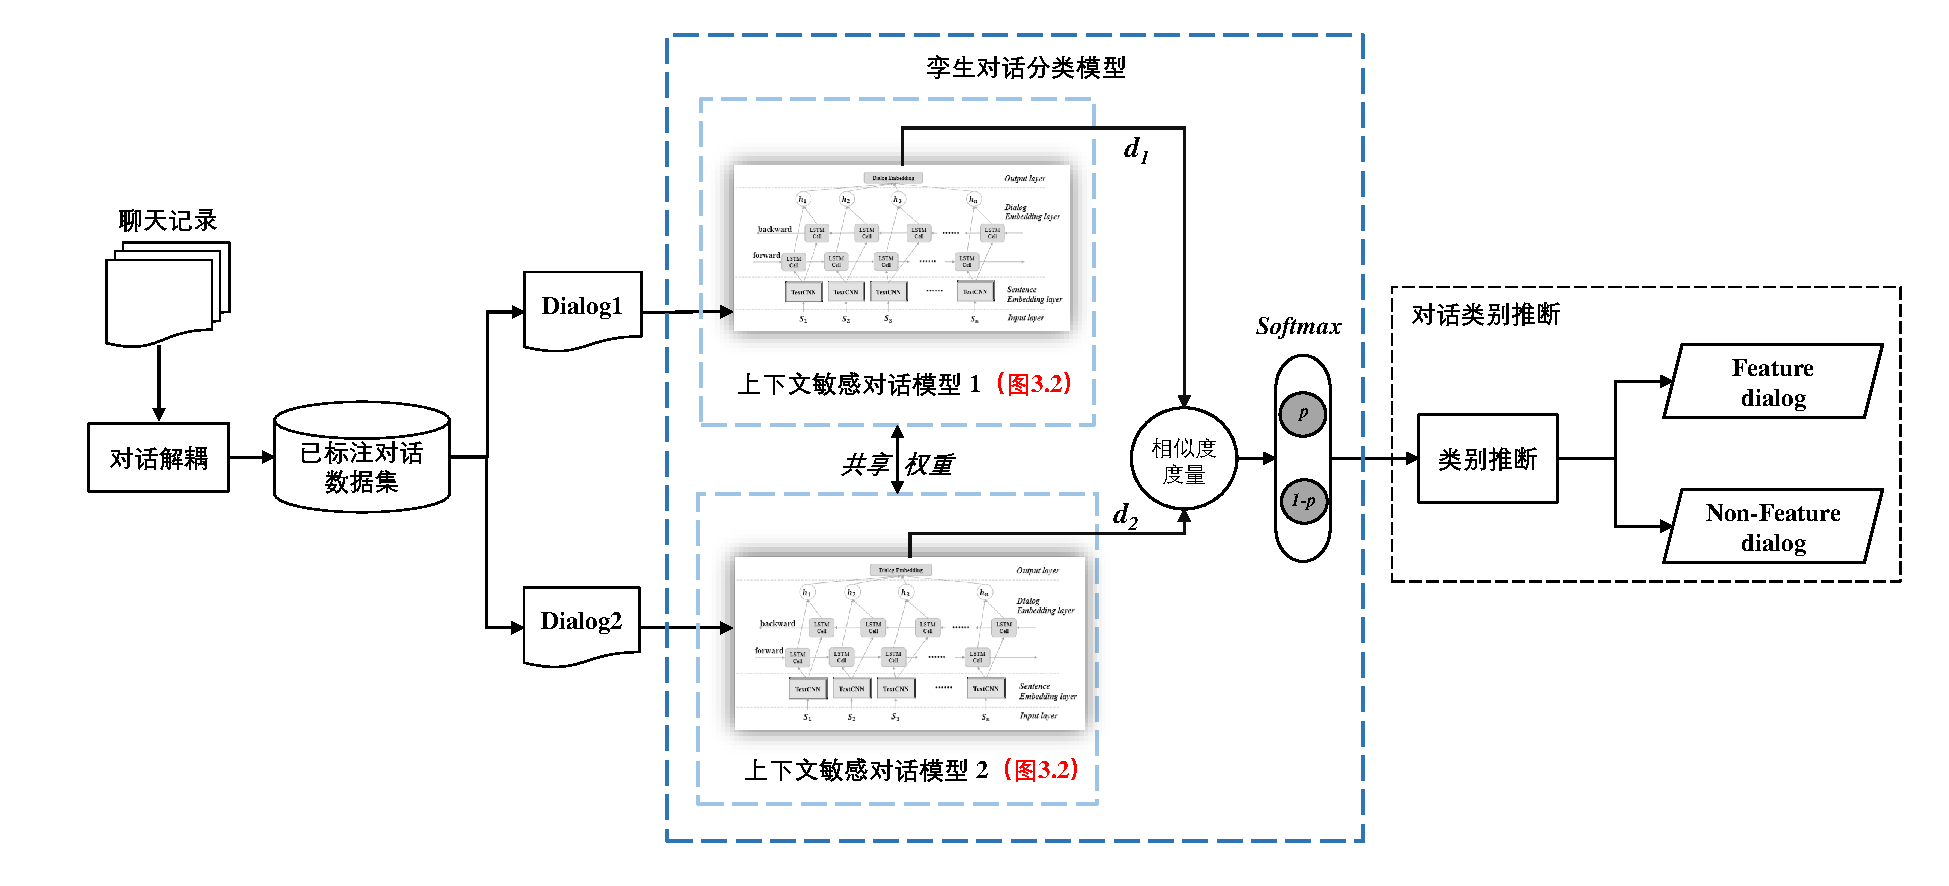
\includegraphics[width=\textwidth]{Img/approach.pdf}
    \bicaption{FRMiner模型结构图}{Architecture of FRMiner}
    \label{fig:approach}
\end{figure}

\section{构建上下文敏感对话模型}
我们设计了一个分层的上下文对话模型,该模型可以捕获上下文信息以及对话中每个句子的语义。如图\ref{fig:model}所示,上下文感知对话模型由四层组成:输入层,句子嵌入层,对话嵌入层和输出层。
\begin{figure}[htbp]
    \centering
    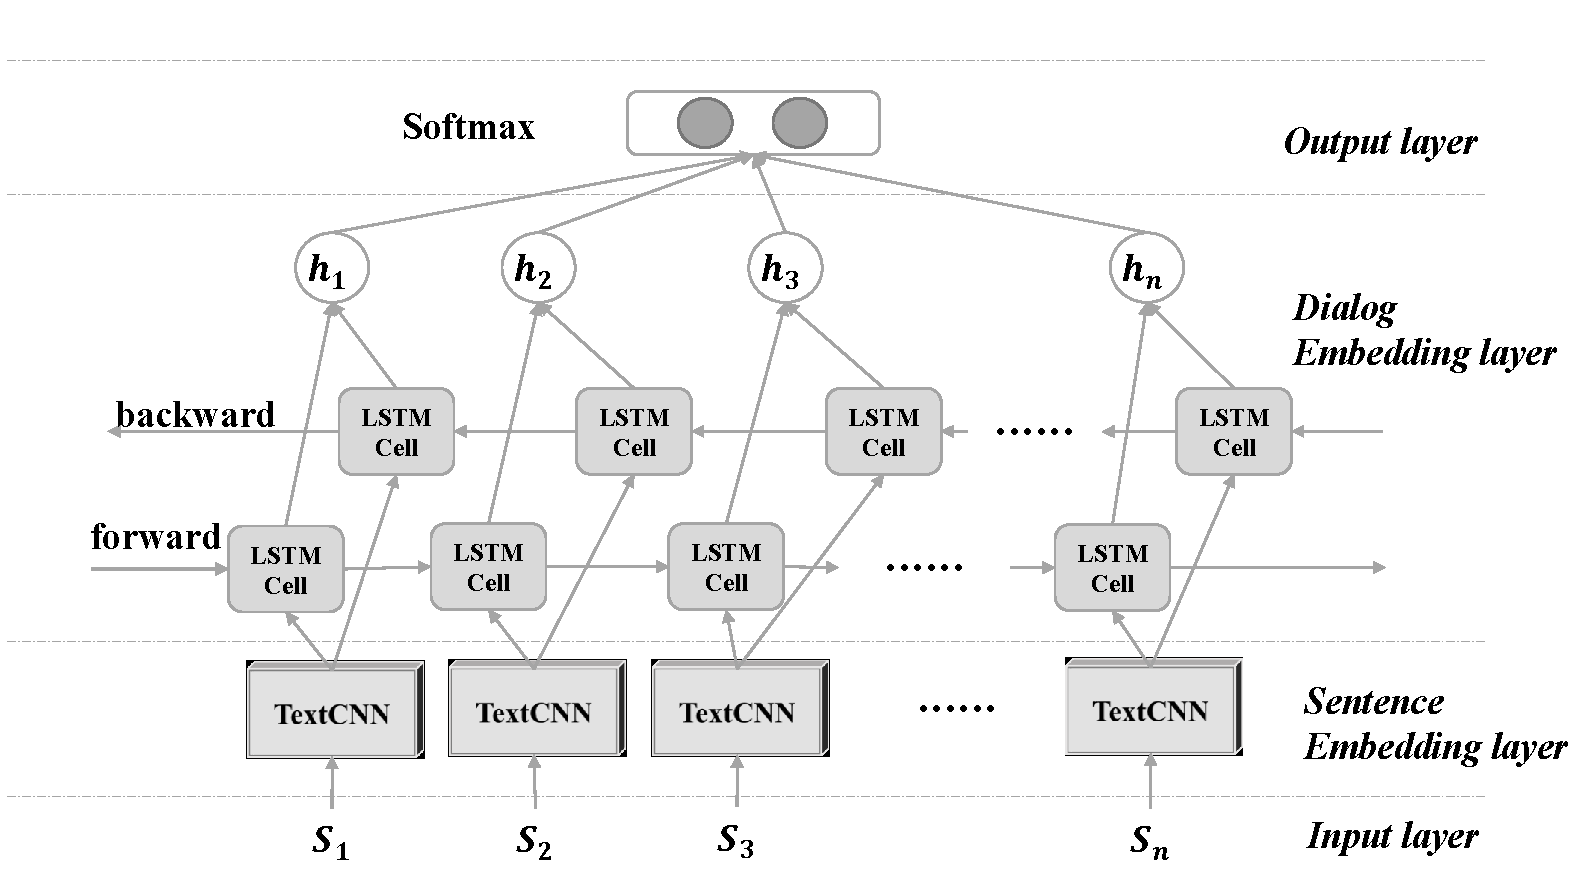
\includegraphics[width=\textwidth]{Img/model.pdf}
    \bicaption{分层的上下文敏感对话模型}{Hierarchical Context-aware Dialog Model}
    \label{fig:model}
\end{figure}

\textbf{输入层:}我们首先将句子分词作为基本元素。为了获得更好的效果,我们利用预先在Wikipedia和Gigword语料库上的60亿个单词上经过训练的50维Glove单词向量\cite{pennington2014glove}作为相应单词的初始向量。此外,受先前工作的启发\cite{Sorbo2016Development} \cite{shi2017understanding},我们注意到特征请求文本中显式地存在词性(POS)模式或模板。直观上,pos-tag可以通过引入显式词汇信息来帮助语义理解。因此,我们将pos-tag信息添加到单词表示中以增强其信息表达。具体来说,每种类型的pos-tag都将初始化为具有均匀分布的随机向量,并在训练过程中进行优化。因此,每个单词可以表示为$w_i=[we_i\oplus pos_i]$,其中$we_i$表示相应的单词嵌入表示,而$pos_i$表示该单词的pos-tag的嵌入表示。

\textbf{句子表示层:}将原始句子转换为单词嵌入和pos-tag嵌入拼接的矩阵后,我们将嵌入表达矩阵输入TextCNN以获取句子表示形式。

\textbf{对话表示层:}在对话表示层中,我们使用一系列句子嵌入来表示对话。当把句子根据对话中的顺序输入BiLSTM编码器时,每个嵌入表达的句子都被当作基本单元。在对BiLSTM进行编码之后,我们可以学习对话的双向上下文信息。

\textbf{输出层:}在输出层中,我们组合由BiLSTM编码的两个方向表示$\overrightarrow{h}$和$\overleftarrow{h}$作为对话的输出向量,其可以表示为$h=[\overrightarrow{h}\oplus \overleftarrow{h}]$。

\section{构建孪生网络分类模型}
为了缓解标记数据不足的问题,我们构建了对话分类孪生网络,将传统的将单个对话映射到其类别的文本分类任务转换为确定两个对话是否属于同一类或不同类的任务,同时扩充数据集。为了清楚起见,在本文的其余部分中,我们将使用\textit{feature dialog}和\textit{non-feature dialog}来表示特征请求的对话和不是特征请求的对话。图\ref{fig:approach}中“3.3”的虚线框显示了详细的体系结构。对话分类孪生网络包含两个上下文感知对话模型,它们共享结构和参数,并将一对对话分别编码为$d_1$和$d_2$。我们使用$d_1$和$d_2$的组合形式$[{d_1}\oplus {d_2}]$来表示两个对话之间的关系。然后将一对对话之间关系的表示从对话嵌入式表示映射为相似度度量。由于用于相似度度量的显式函数(例如余弦相似度和欧几里得距离\cite{huang2008similarity})通常用于测量线性空间中向量之间的接近度,因此它们不适用于语义空间中的复杂对话。因此,我们采用在训练神经网络过程中学习到的相似性函数。由于可以获得两个对话是否相似的标签,因此我们可以据此训练神经网络中的相似层。它就像一个黑匣子模块,输入是带有\textit{same}或\textit{diff}标签的两个对话的嵌入式表示,输出是它们的相似性。

我们按照以下步骤训练对话分类孪生网络。
\begin{enumerate}
    \item 我们将数据集随机分为训练和测试数据集。\textit{Train\_d}是原始数据集,它使用带有标签\textit{feature dialog}或\textit{non-feature dialog}的对话作为基本数据单元。
    \item 通常,标注对话的大小不足以训练有效的基于有监督学习的模型。为了解决该问题,我们通过采样来自\textit{Train\_d}的一对对话作为\textit{Train\_p}(标签为\textit{same}或\textit{diff})的一个基本数据单元,将\textit{Train\_d}数据集增强为\textit{Train\_p}。更具体地说,对于训练数据集中的每个对话,我们从训练数据集\textit{Train\_d}中分别随机选择一个带有\textit{feature dialog}标签的正样本和一个带有\textit{non-feature dialog}标签的负样本。例如,如果两个对话都是\textit{feature dialog}或\textit{non-feature dialog},我们将为它们分配标签——\textit{same},否则为\textit{diff}。由于采用一正一负的抽样策略,我们的训练数据可以天然地进行数据平衡。此外,假设我们在\textit{Train\_d}中有 $m$ 个特征请求对话和$n$个非特征请求对话,我们可以将原始数据集扩展为 $\tbinom{m}{2}+\tbinom{n}{2}+m\times n$。但是此种数据增强方式的数据量过大,为了减小数据增强后数据集规模同时又不能增大随机采样带来的误差,我们对以上流程在整个数据集上及进行$iter\_num$次。伪代码如算法\ref{alg:trainset}所示:
    \begin{algorithm}[htbp]
            \caption{FRMiner Pair-Instance训练集构建算法}  
            \label{alg:trainset}
            \begin{algorithmic}[1]
                \Require list 正样本集合 Pos,list 负样本集合 Neg, int 迭代次数 iter\_num 
                \Ensure list <pair> 训练集 
                \Function{pair\_instance}{list Pos, list Neg, int iter\_num} 
                    \State pairs \gets [\ ]
                    \For {i\ in\ range(iter\_num)}
                        \For {d\ \in\ Pos\ \cup\ Neg}
                            \State p \gets random(Pos)
                            \State n \gets random(Neg)
                            \State pairs.append(<d,\ p>)
                            \State pairs.append(<d,\ n>)
                        \EndFor
                    \EndFor
                    \State \Return $pairs$
                \EndFunction  
            \end{algorithmic}  
    \end{algorithm}
    \item 最后,由于每对对话都属于\textit{same}类或\textit{diff}类,因此相似性度量的输出为长度为2的向量$[score_1 , score_2]$  ,代表两个类的分数,其中$score_i \in \mathbb{R}$ 。 我们对此向量执行softmax,可以表示为
    $$Softmax(socre_i)=\frac{e^{score_i}}{\sum_{j=1}^2 e^{score_j}}$$ 
    ,然后可以将 $[score_1 , score_2]$ 归一化为概率$[p ,1-p]$,其中 $p \in [0,1]$。
\end{enumerate}
\section{分类概率推断}
对话分类孪生网络的输出是表示两个对话是相似还是不相似的概率。但是我们需要的是对话是否为特征请求对话的概率,因此,我们需要基于对话的概率和配对对话的实际标签来推断此对话的标签。例如,我们采样一对$<Dialog_1,Dialog_2>$ ,其中 $Dialog_1$ 是从训练数据集中采样的有标签对话,其标签为\textit{non-feature dialog},而 $Dialog_2$是要预测的未知对话。我们将它们输入到对话分类孪生网络中,然后做出两个对话为相似或不相似的预测。假设预测为不相似,则可以推断出$Dialog_2$ 的类为\textit{feature dialog}。如果$Dialog_2$ 的实际标签是\textit{feature dialog},则表明我们的模型做出的这种预测是正确的。否则,我们的预测结果是假阳的。为了获得更可靠的预测结果,我们在预测阶段时采用了投票策略。对于每个未知标签对话,我们通过对$k$个不同的有标签对话进行采样来构造$k$个配对样本。将这些对传递到FRMiner后,基于FRMiner的预测结果和有标签对话的标签,我们可以得到$l$个样本指示未知标签对话为\textit{feature dialog}和$k-l$个样本指示未知标签对话为\textit{non-feature dialog}。如果$l$大于$\frac{k}{2}$,则为预测的对话标注为\textit{feature dialog}标签,反之亦然。伪代码如算法\ref{alg:infer}所示:
    \begin{algorithm}[htbp]
            \caption{测试阶段分类类别Inference算法}  
            \label{alg:infer}
            \begin{algorithmic}[1]
                \Require list 训练样本集 train,list 测试样本集 test
                \Function{test\_infer}{list train, list test} 
                    \For{t\ in\ test}
                    \State golden \gets random(train)
                    \State p \gets FRMiner(<t,\ golden>)
                    \If {p\ is\ 'same'}
                        \If {golden.label\ is\ 'feature'}
                        \State t.label \gets 'feature'
                        \EndIf
                        \If {golden.label\ is\ 'non-feature'}
                        \State t.label \gets 'non-feature'
                        \EndIf
                    \EndIf
                    \If {p\ is\ 'diff'}
                        \If {golden.label\ is\ 'feature'}
                        \State t.label \gets 'non-feature'
                        \EndIf
                        \If {golden.label\ is\ 'non-feature'}
                        \State t.label \gets 'feature'
                        \EndIf
                    \EndIf
                    \EndFor
                \EndFunction  
            \end{algorithmic}  
    \end{algorithm}
\section{本章小结}